\chapter{Design} \label{chapter:design}
This chapter presents the design process for the system, including architectural choices and the rationale behind them. The design is guided by the requirements from the previous chapter.


\section{Design Context}
This project is based on two primary data sources: robotic programs developed for Universal Robots systems and technical documentation from the robot manufacturer. These data sources represent both concrete implementations of robotic tasks and contextual knowledge about robot capabilities and programming concepts.

\subsection{Robot Programs}
The robotic programs, in the Universal Robots \texttt{.urpx} format, represents a complete robot program. Internally, these files follow a structured, hierarchical format that resembles JSON. The structured nature of the \texttt{.urpx} files allows for systematic extraction of metadata describing the semantics of the program. For this theis, it is assumed that every program file is associated with a metadata file that characterizes the program. A similar metadata file is eventually expected to be available from the FERA program repository as well. This metadata includes attributes such as the application type, actions performed, and the hardware context e.g., robot model and end-effector type.

The following (see Code~\ref{listing:design:data_robot_programs}) shows the JSON structure of the program metadata.
\begin{listing}[h]
    \begin{minted}{json}
                            {
                                "id": "integer",
                                "name": "string",
                                "robotType": "string",
                                "applicationType": "string",
                                "gripperType": ["string"],
                                "image": "string",
                                "dataAvailable": "string",
                                "components": "string",
                                "program": "string",
                                "additionalImage": "string",
                                "totalRating": "integer",
                                "ratingCount": "integer",
                                "objectType": ["string"],
                                "objectWeight": "number",
                                "cncDoorControl": "boolean",
                                "communicationType": "string",
                                "actions": ["string"]
                            }
    \end{minted}
    \caption{JSON structure of robotic program metadata.}
    \label{listing:design:data_robot_programs}
\end{listing}

\subsection{Robot Documentation}
In addition to program data, technical documentation is available in \texttt{.pdf} format. This documentation includes manuals, guidelines, and reference materials from the Universal Robots documentation portal. \cite{UniversalRobots2026Downloads} Each documentation file contains upward of hundreds of pages of information. Unlike robotic programs, which are structured artifacts, documentation represents unstructured textual data that provides explanatory and contextual information about robot functionality and programming concepts.


\newpage
\section{Architectural Design}
As presented in Chapter~\ref{chapter:related-work}, recent advances in LLMs and AI assistants have demonstrated strong potential within software engineering, where they are increasingly used for tasks such as code generation, question answering, debugging, and code modification. We explore how similar assistant-based approaches can support robotic program development.

The functional requirements (see Section~\ref{sec:requirement_engineering:specification}) of the system specify capabilities beyond standalone language generation. Tasks such as answering questions about robotic programs, generating or modifying code, and debugging robot programs require the assistant to have agentic capabilities to efficiently support the developer. For example, answering a question about a robotic program may require grounding the response in relevant documentation. Modifying a robot program may require inspecting the program and understanding the existing code, iteratively refining the modification based on feedback, and validating the modified program.

Consequently, the assistant should be augmented with a set of tools that enable these functional requirements. Rather than acting only as a static response generator, it should support an interactive workflow in which external tools can be used whenever a user query requires it.

The assistant would ideally have access to multiple categories of tools that support different stages of the robotic program development workflow. Retrieval tools would enable access to technical documentation and previously developed robotic programs relevant to the user's query. Program inspection tools would allow the assistant to analyze program structure, metadata, and control flow directly from the underlying robotic artifacts, enabling reasoning grounded in the program itself rather. Modification tools would support structured editing and transformation of programs. Verification tools, including syntax checkers, schema validators, and static analysis utilities, would support validation of generated modifications. Simulation tools could enable evaluation of generated changes against expected robot behavior in controlled environments prior to execution on physical systems. Collectively, these tool categories support the broader development workflow of retrieval, comprehension, modification, verification, and validation of robotic programs.

However, use of such tools depends on the user query and requires an architecture that supports agentic behavior. The assistant must be able to decide when to use tools, which tools to use, and how to integrate tool output into its reasoning and response generation. Thus, the assistant architecture adopted in this project is inspired by the ReAct framework (also mentioned in Chapter~\ref{chapter:related-work}), in which a language model iteratively alternates between reasoning about a task and invoking external tools to gather information or perform actions. This approach is well suited for robotic program development tasks because user requests may require multiple intermediate steps before a suitable response can be generated.

Figure \ref{fig:design:agentic_orchestration_flowchart} shows the agentic orchestration loop architecture and illustrates how reasoning, tool use, evidence evaluation, and response synthesis are connected.

\begin{figure}[H]
    \centering
    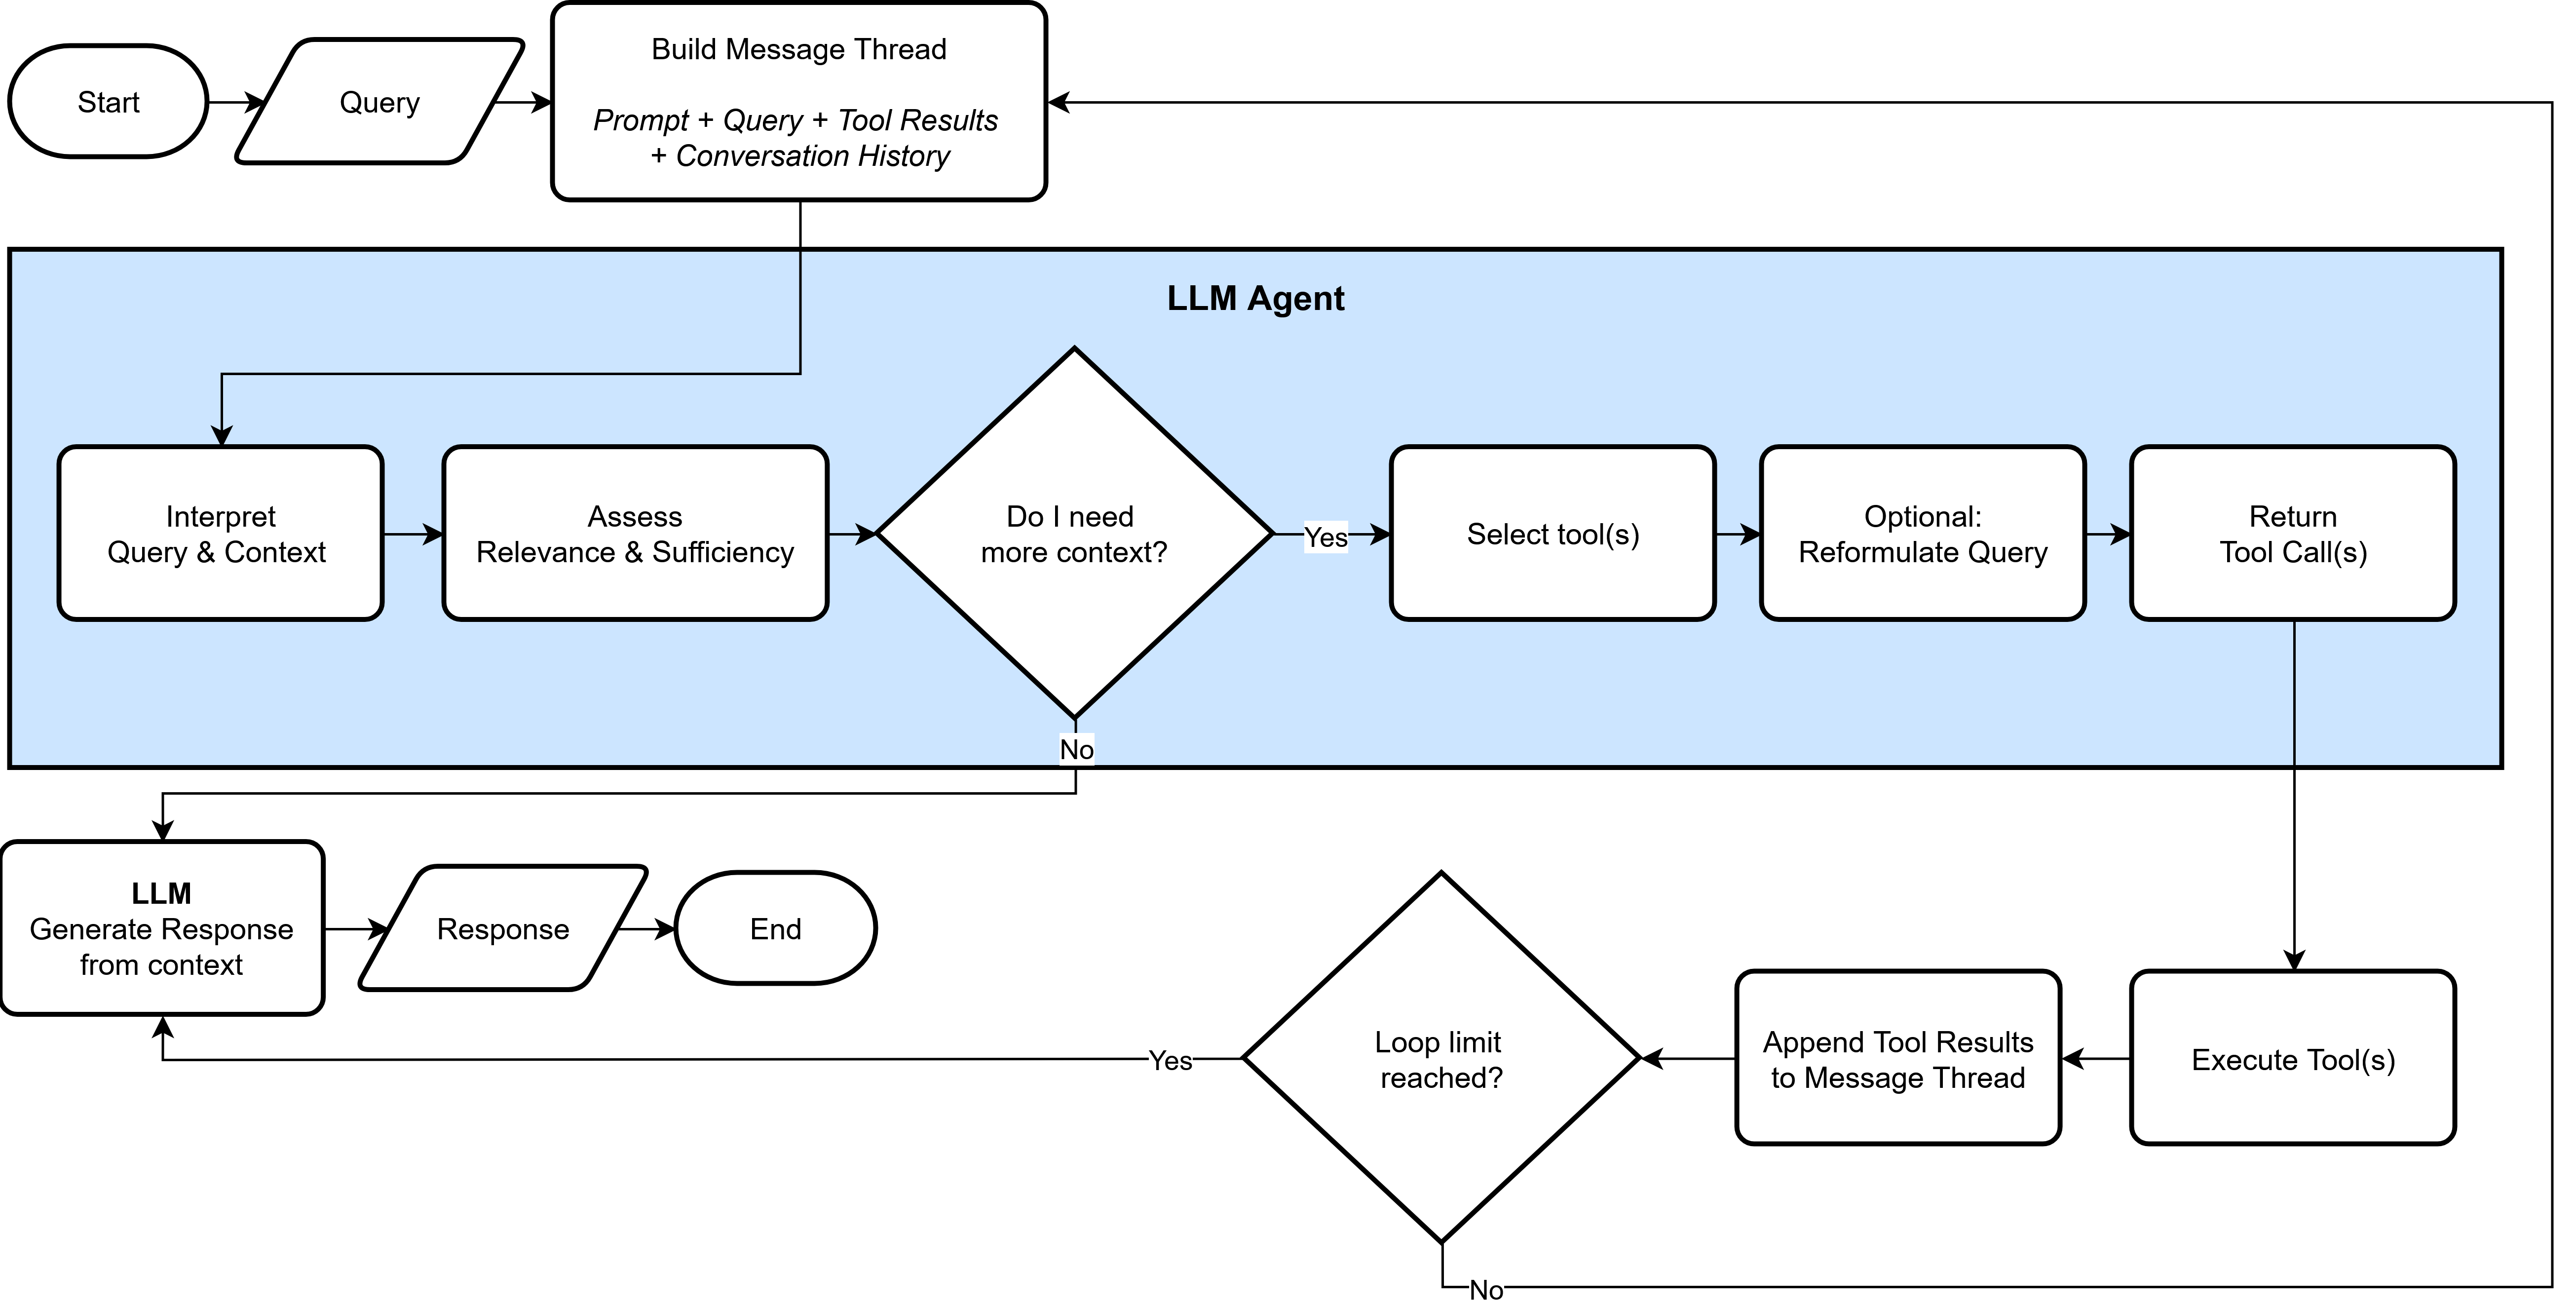
\includegraphics[width=\columnwidth]{media/orchestration-flowchart.png}
    \caption{{Agentic orchestration loop flowchart.}}
    \label{fig:design:agentic_orchestration_flowchart}
\end{figure}

Within this architecture, a language model acts as the orchestration component responsible for interpreting user requests, selecting appropriate tools, reasoning over retrieved information and generating responses. Having multiple specialized LLMs for different roles e.g., one for orchestration and another for response generation, could result in better performance and quality because each model can be optimized for its specific purpose. However, to take full advantage of this, we would have to train or fine-tuning domain-specific models, which is not feasible given the scope of the project and the available data. Therefore, the design of the system should for now use general-purpose LLMs for both orchestration and response generation, and the focus should be on augmenting these models with the necessary tools and retrieval capabilities to support robotic program development tasks. This design allows the system to leverage the general reasoning and language capabilities of existing LLMs, while future work can explore the potential benefits of domain-specific training or fine-tuning for improved performance in robotic programming contexts.

Due to the scope of this thesis, the following system design focuses primarily on retrieval-based tools for integrating the available robotic knowledge sources into the assistant's reasoning process. Additional tools are discussed as directions for future work in Chapter~\ref{sec:discussion:future-work}.


\newpage
\section{Retrieval-Augmented Generation (RAG)}
As discussed in Section~\ref{sec:related-work:RAG}, retrieval-augmented generation extends a language model with access to external knowledge. This allows the integration of the robotic domain knowledge into the general language model to ground its responses in up-to-date and relevant information, without requiring the model itself to be retrained whenever the knowledge base changes. It also supports transparency, because retrieved context can be traced back to its source.

Figure~\ref{fig:design:rag} illustrates this overall retrieval-augmented generation pattern, in which external knowledge is retrieved and incorporated into the model context before response synthesis.

\begin{figure}[H]
    \centering
    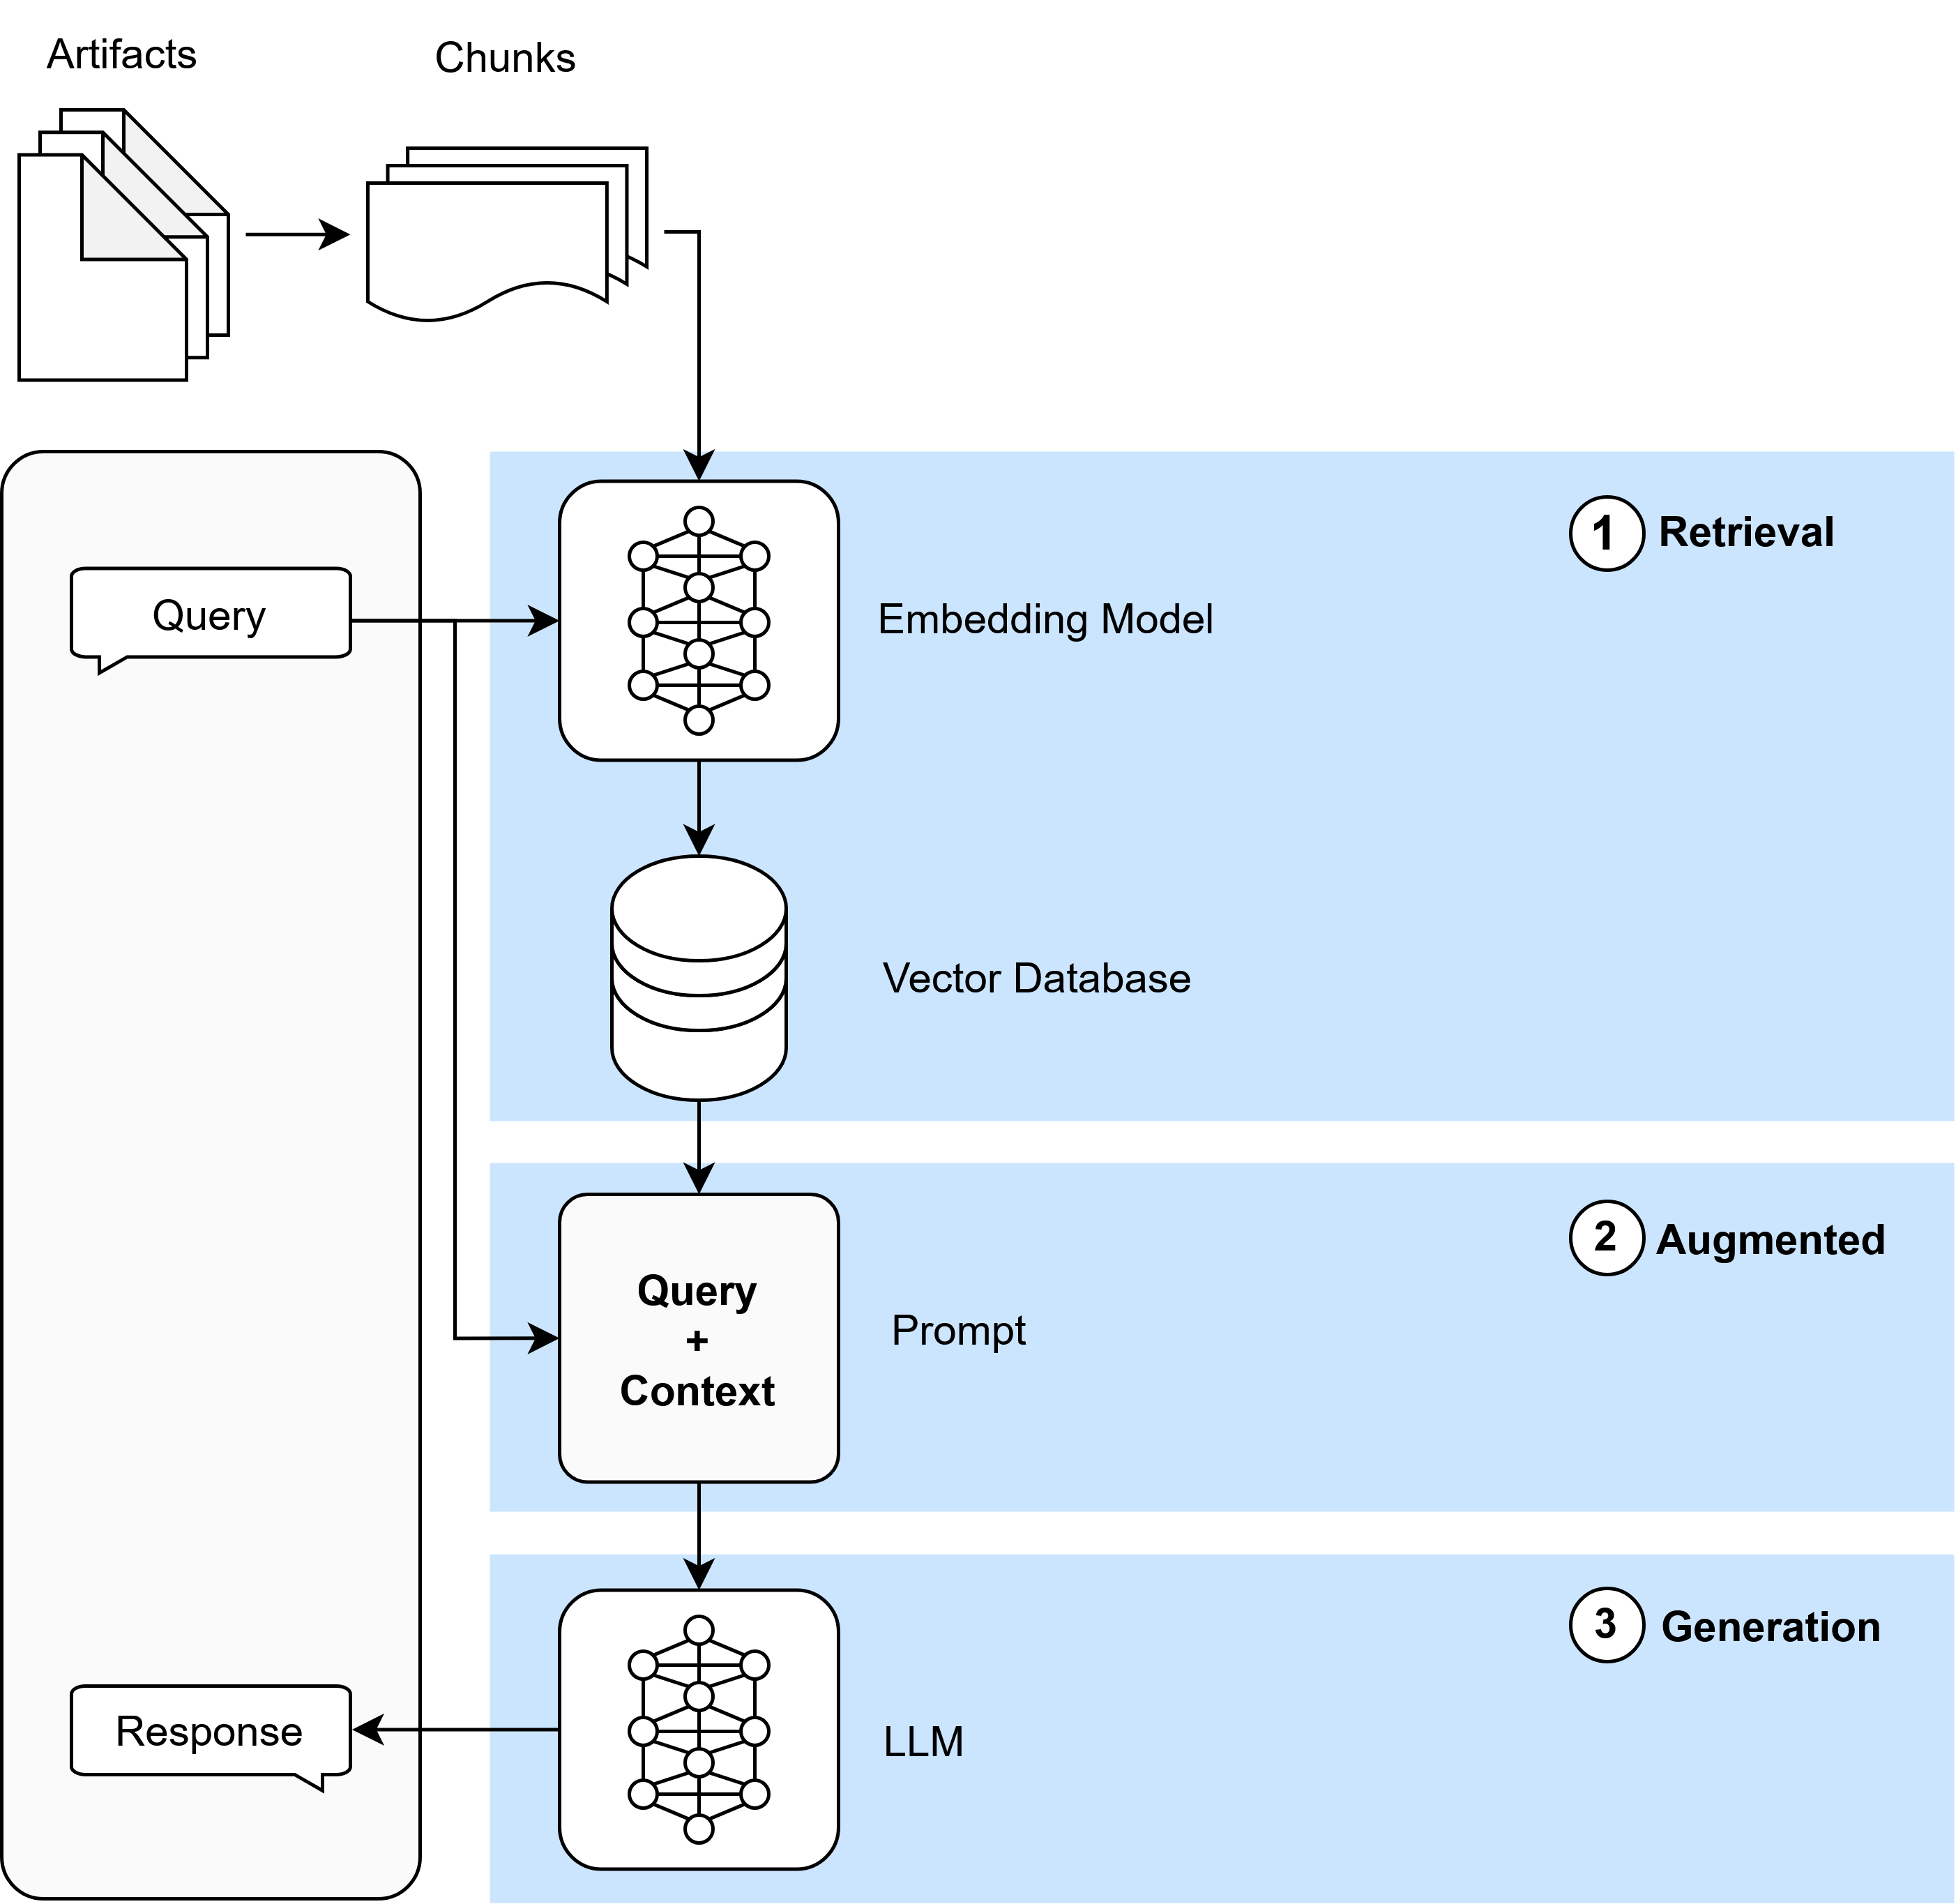
\includegraphics[width=0.8\columnwidth]{media/rag.png}
    \caption{{Retrieval-Augmented Generation (RAG).}}
    \label{fig:design:rag}
\end{figure}


In Section~\ref{sec:related-work:RAG}, several RAG variants were presented, naive RAG, advanced RAG, modular RAG, and agentic RAG. Agentic RAG overlaps with the ReAct-style agentic orchestration loop described above, as both emphasize the role of retrieval as an explicit tool-mediated action within the reasoning loop. This design allows the assistant to adaptively decide when and how to retrieve evidence based on the evolving context of the interaction, rather than relying on a fixed retrieval step before response generation. The overlap means that providing the orchestration agent with retrieval tools effectively implements an agentic RAG architecture, where retrieval is integrated into the assistant's reasoning process in a flexible and context-sensitive way.

\subsection{Retrieval}
The retrieval mechanism is designed around semantic search, in which user queries and indexed artifacts are represented in a shared semantic space. Rather than depending solely on exact keyword overlap, the system can identify programs and documentation passages whose meaning is close to the user's intent. This is well suited to the present domain because users formulate requests in natural language, whereas the underlying sources contain robotics-specific terminology, structured metadata, and implementation details that may not share the same vocabulary.

Alternative strategies were considered. Exact keyword search is effective when the user's terminology closely matches the corpus, but it performs poorly when the same concept is expressed using different words. However, hybrid retrieval, combining semantic similarity with keyword constraints, remains a relevant extension for cases where exact identifiers or parameter names are important.

Figure \ref{fig:design:semantic_search} illustrates the semantic search approach adopted in the system.

\begin{figure}[H]
    \centering
    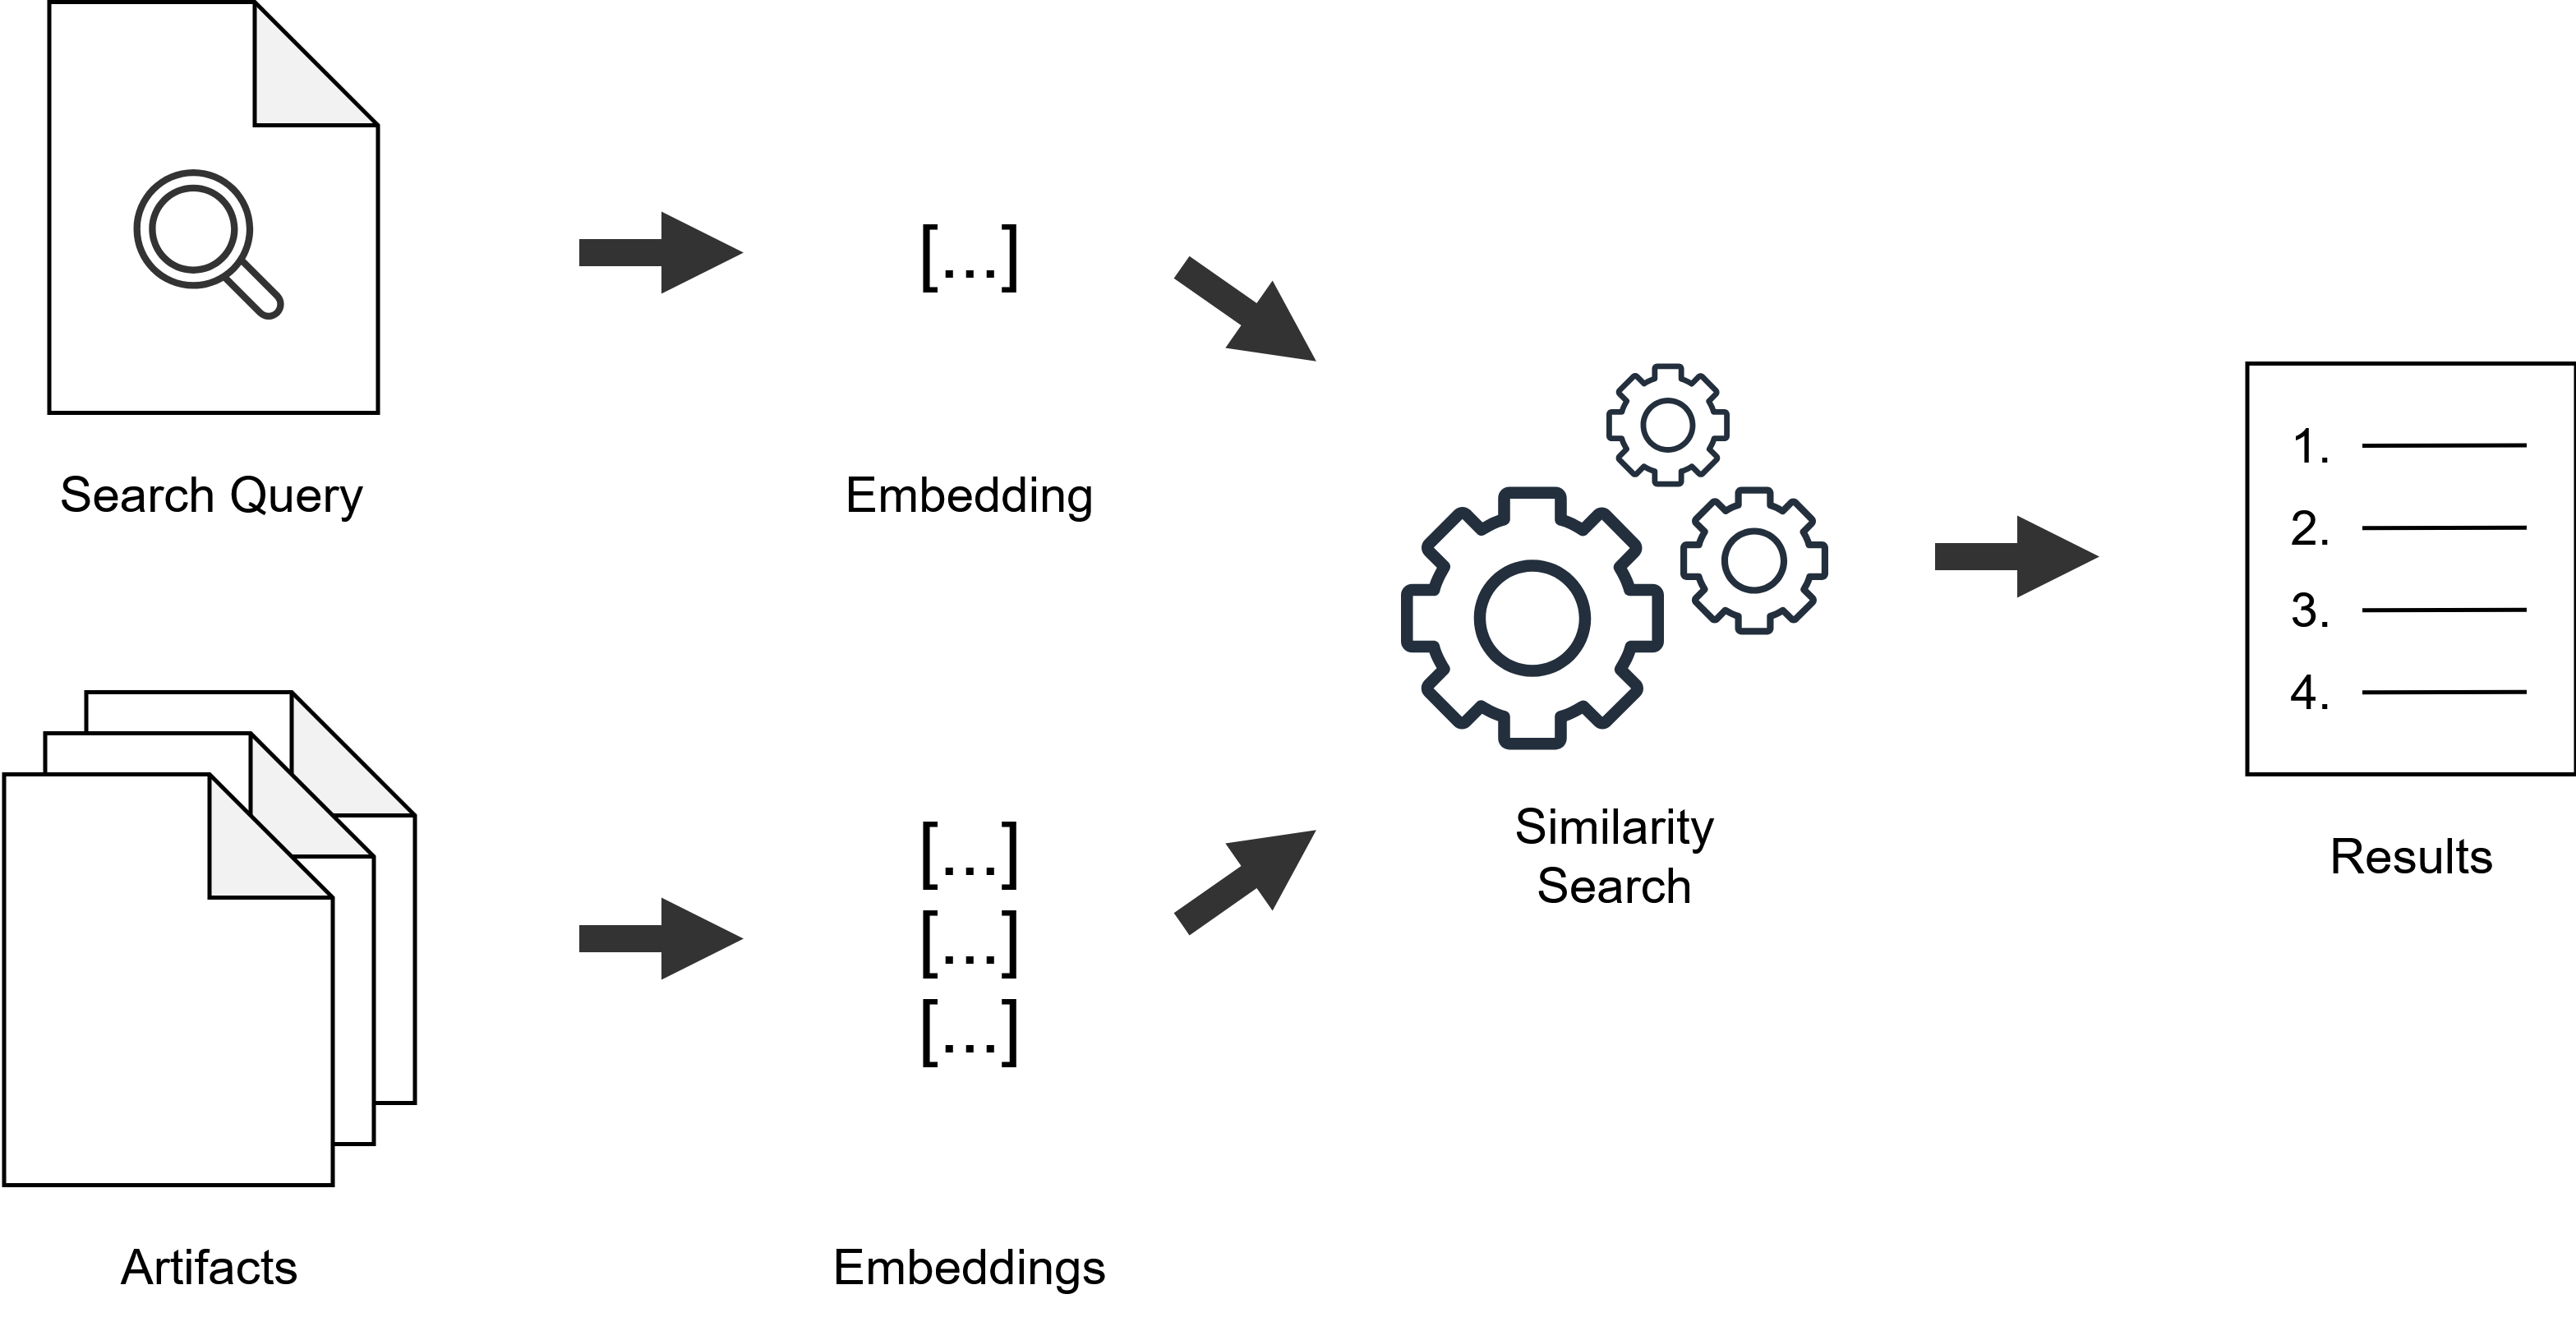
\includegraphics[width=0.8\columnwidth]{media/semantic_search.png}
    \caption{{Semantic Search.}}
    \label{fig:design:semantic_search}
\end{figure}


\subsection{Data Pipeline}
RAG depends on external knowledge being available in a form that can be retrieved efficiently at runtime. In this thesis, those knowledge sources are program metadata, robot program code, and documentation. The data pipeline should therefore convert these raw sources into retrieval-oriented representations, embed those representations, and organize them in a way that supports efficient semantic search. The quality of this pipeline directly affects how well the assistant can identify and use relevant sources during interaction.

These data sources should be preserved as separate representations, opposed to being merged into a single undifferentiated retrieval space, because they serve different roles in the assistant workflow. Metadata-oriented program summaries support discovery of relevant examples, program-code chunks provide structural detail for comprehension and modification tasks, and documentation chunks contribute explanatory knowledge. Keeping these sources separate improves retrieval controllability and makes it easier to combine evidence deliberately during response generation.

The data pipeline should operate as an offline preparation layer so that computationally expensive transformation, chunking, and embedding operations do not have to be performed during user interaction. This improves runtime responsiveness and preserves modularity, since chunking strategies, embedding models, and ingestion processes can be refined independently of the assistant's orchestration logic.

Figure \ref{fig:design:data_ingestion} illustrates the data pipeline, which consists of three stages: data transformation, embedding, and ingestion, each discussed in the subsequent subsections.

\begin{figure}[H]
    \centering
    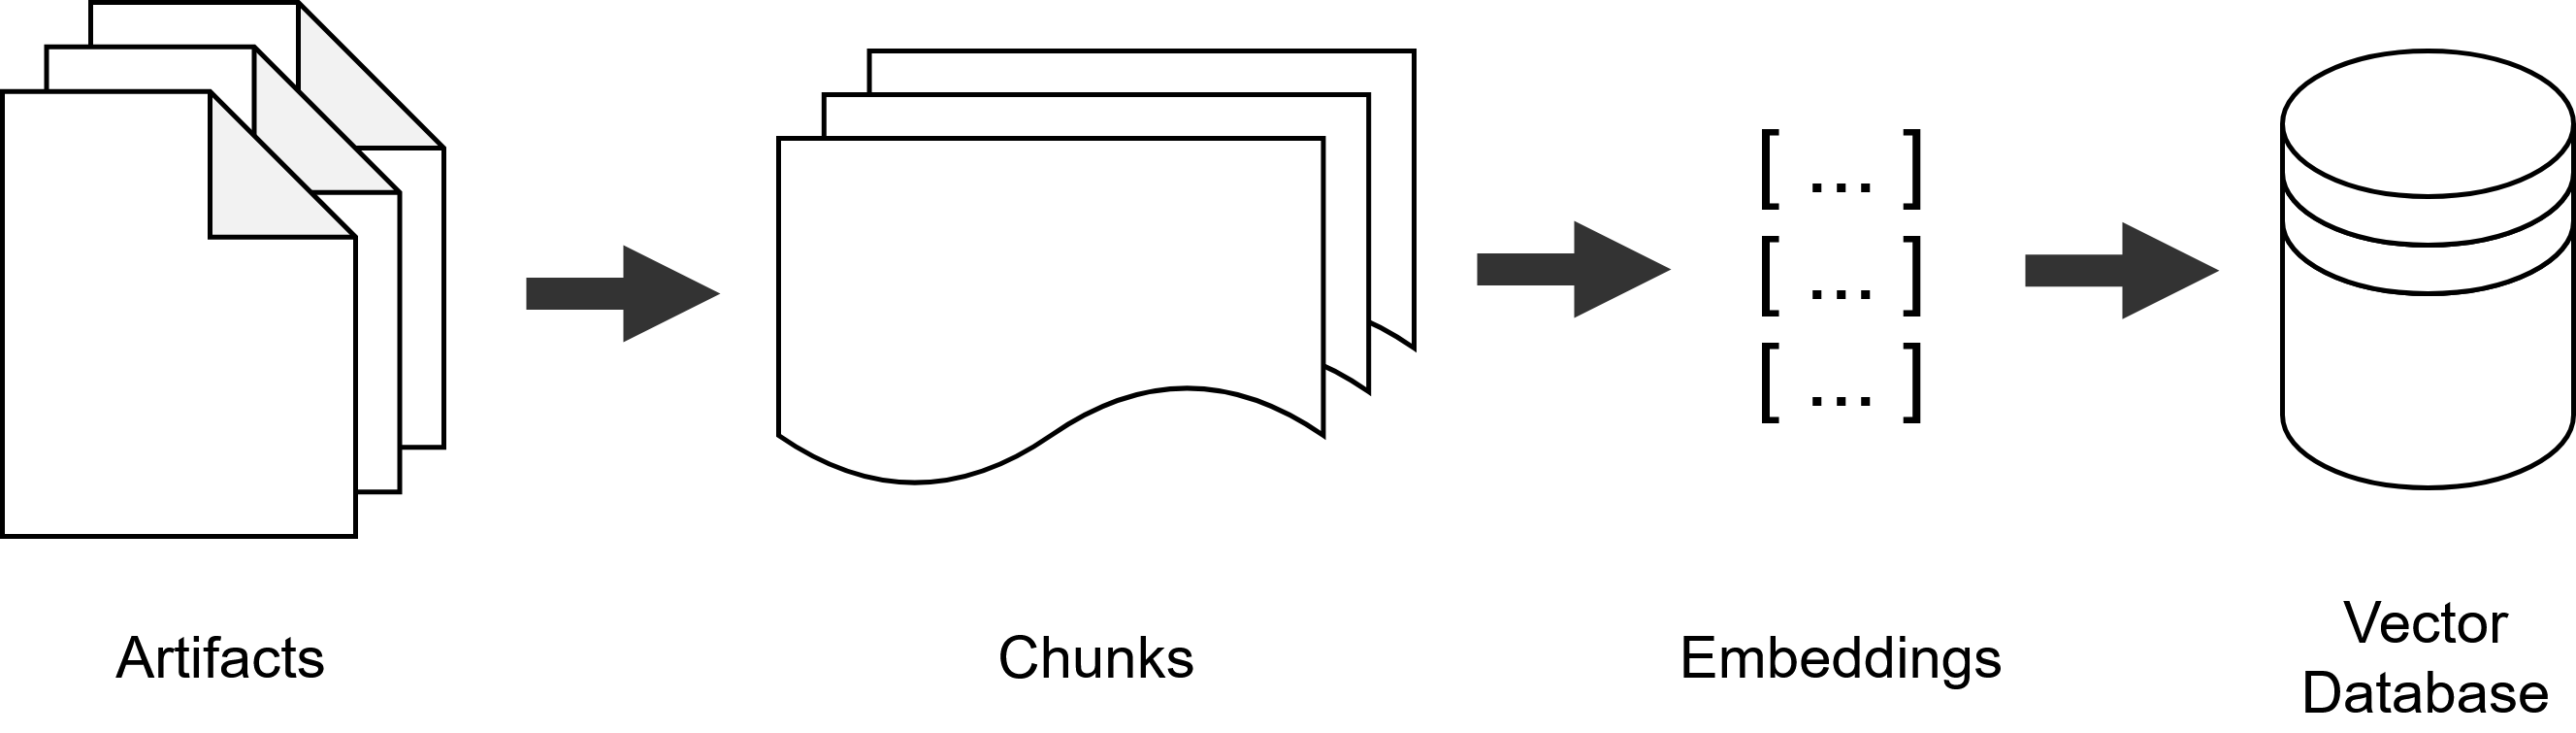
\includegraphics[width=0.9\columnwidth]{media/data_ingestion.png}
    \caption{{Data Pipeline.}}
    \label{fig:design:data_ingestion}
\end{figure}

\subsubsection{Transformation and Chunking}
The system relies on three information sources with different semantic roles. Because these sources differ in structure and purpose, transformation and chunking are designed per source. A critical constraint is the limited context window of language models: entire programs or documentation files quickly exhaust available model context, making it impractical to retrieve full artifacts for synthesis. Chunking is therefore essential to partition large artifacts into focused units that can fit within context limits while preserving semantic coherence. This introduces a design trade-off: finer-grained chunking can improve retrieval precision, but it may fragment context across multiple chunks, whereas coarser chunking preserves more local context at the cost of lower retrieval precision and more irrelevant surrounding material. Additionally, model performance can degrade as the context window fills, making efficient use of limited context, as well as context management, important design concerns. \cite{liu2024lost}

\paragraph{Program Metadata}~\\
Program metadata captures high-level intent, including task type, robot context, components, and actions. During transformation, these structured fields should be converted into concise natural-language representations to align with the behavior of semantic search and embedding models, which generally capture meaning more effectively from textual descriptions than from raw structured syntax. While JSON structures could be embedded directly, this would increase token usage without adding comparable semantic value for retrieval. Metadata-oriented representations are therefore designed for intent-level retrieval, either for identifying programs or for guiding the assistant in reasoning about high-level implementation details.

\paragraph{Program Code}~\\
Program code provides structural details that metadata alone cannot express. The program structures should be transformed into semantically meaningful fragments. As with metadata, structured content is expressed as compact natural-language descriptions, because dense structural encodings increase token volume but often contribute less semantic signal for embedding-based retrieval. Chunking at this level balances precision: shorter chunks enable targeted retrieval of specific operations or patterns, but longer chunks preserve more operational context, which may be needed for modification tasks. The chunking strategy should use structural cues such as node definitions to create coherent units that can be retrieved and reasoned about effectively. This allows the assistant to access relevant code details without overwhelming the model with excessive context.

\paragraph{Documentation}~\\
Documentation is an unstructured source composed of long, multi-topic texts. It should therefore be segmented into coherent chunks that align with local concepts and preserve contextual continuity. A key design consideration for documentation chunking is overlap: adjacent chunks should be permitted to share boundary content (typically a few sentences) so that retrieval at a chunk boundary does not abruptly lose context needed for the synthesis model to reason about the retrieved passage. This sliding-window approach is particularly important for documentation because technical concepts often span multiple sentences, and a sharp chunk boundary can cut sentences short. Chunk boundaries are aligned with structural features, section headers, paragraphs, and topic shifts, rather than fixed token counts, which better preserves semantic coherence. This enables targeted retrieval of relevant explanatory passages instead of entire manuals, which improves precision for technical questions. Less relevant sections e.g. table of contents should be filtered out during transformation to avoid polluting the retrieval space with low-value content.

\subsubsection{Embedding}
Following transformation and chunking, the resulting program representations and documentation chunks should be embedded into dense vector representations to enable semantic similarity search. Embedding the transformed natural-language representations allows user queries to be matched against robotic programs and documentation based on semantic meaning.

\subsubsection{Ingestion}
Ingestion is the final preparation stage in which the embedded representations are written into the retrieval layer together with the metadata needed to use them effectively at runtime The ingestion design decides how the assistant's knowledge is organized and exposed to retrieval, and therefore determines which kinds of evidence can be retrieved, how they are distinguished from one another, and how they can later be traced back to their sources.

The system should preserve the three evidence types as separate representations: metadata representations, code-level program chunks, and documentation chunks. This separation reflects their different roles in the assistant workflow. Metadata-oriented program representations support retrieval of relevant robotic solutions at the task level, program-code chunks provide structural detail for comprehension and modification, and documentation chunks contribute explanatory knowledge. Keeping these representations separate improves retrieval control.

Ingestion should also preserve provenance. Each ingested entry should retain source identity and linking information to the underlying artifact from which it was derived. This is particularly important for robotic programs and metadata, where the semantic representations are useful for retrieval, but the original structured artifacts are required during reasoning and response generation. This also allows the assistant to trace retrieved evidence back to its source, which supports transparency and enables the user to inspect the original artifact when needed.


\section{Frontend}
\subsection{User Interface}
The user interface forms the primary interaction point between the developer and the assistant, and its design therefore plays an important role in how effectively the assistant can support robotic program development tasks. The interface should expose the assistant's capabilities in a way that supports both exploration of existing robotic solutions and focused comprehension and modification of individual programs.

These activities place different demands on the interface and should therefore be separated into distinct workspaces. Search-oriented workflows benefit from lightweight navigation across many candidate programs, whereas comprehension and modification tasks require sustained attention to a single artifact together with supporting contextual information. The frontend design therefore separates interaction into a search workspace and an editor workspace.

A web-based frontend was selected to align with both the expected FERA platform architecture and modern robotics software environments such as PolyScope X, which are themselves web-oriented. Since the assistant is intended to support workflows within these environments, adopting a compatible frontend architecture simplifies potential integration and promotes consistency across systems. In addition, web applications are platform-independent and support distributed system architectures in which frontend, backend, retrieval infrastructure, and language-model orchestration remain separated components communicating through network interfaces. Modern web technologies are also well suited for AI-assisted interaction patterns, including conversational interfaces, asynchronous communication, and streaming responses.

Figures~\ref{fig:design:lofi_search} and \ref{fig:design:lofi_edit} present low-fidelity wireframes for the two workspaces. The search workspace shown in Figure~\ref{fig:design:lofi_search} prioritizes natural-language querying and inspection of ranked program results. Users should be able to compare candidate programs based on semantic descriptions and metadata before loading a specific artifact into the editor workspace. This supports efficient discovery of relevant robotic solutions.

\begin{figure}[H]
    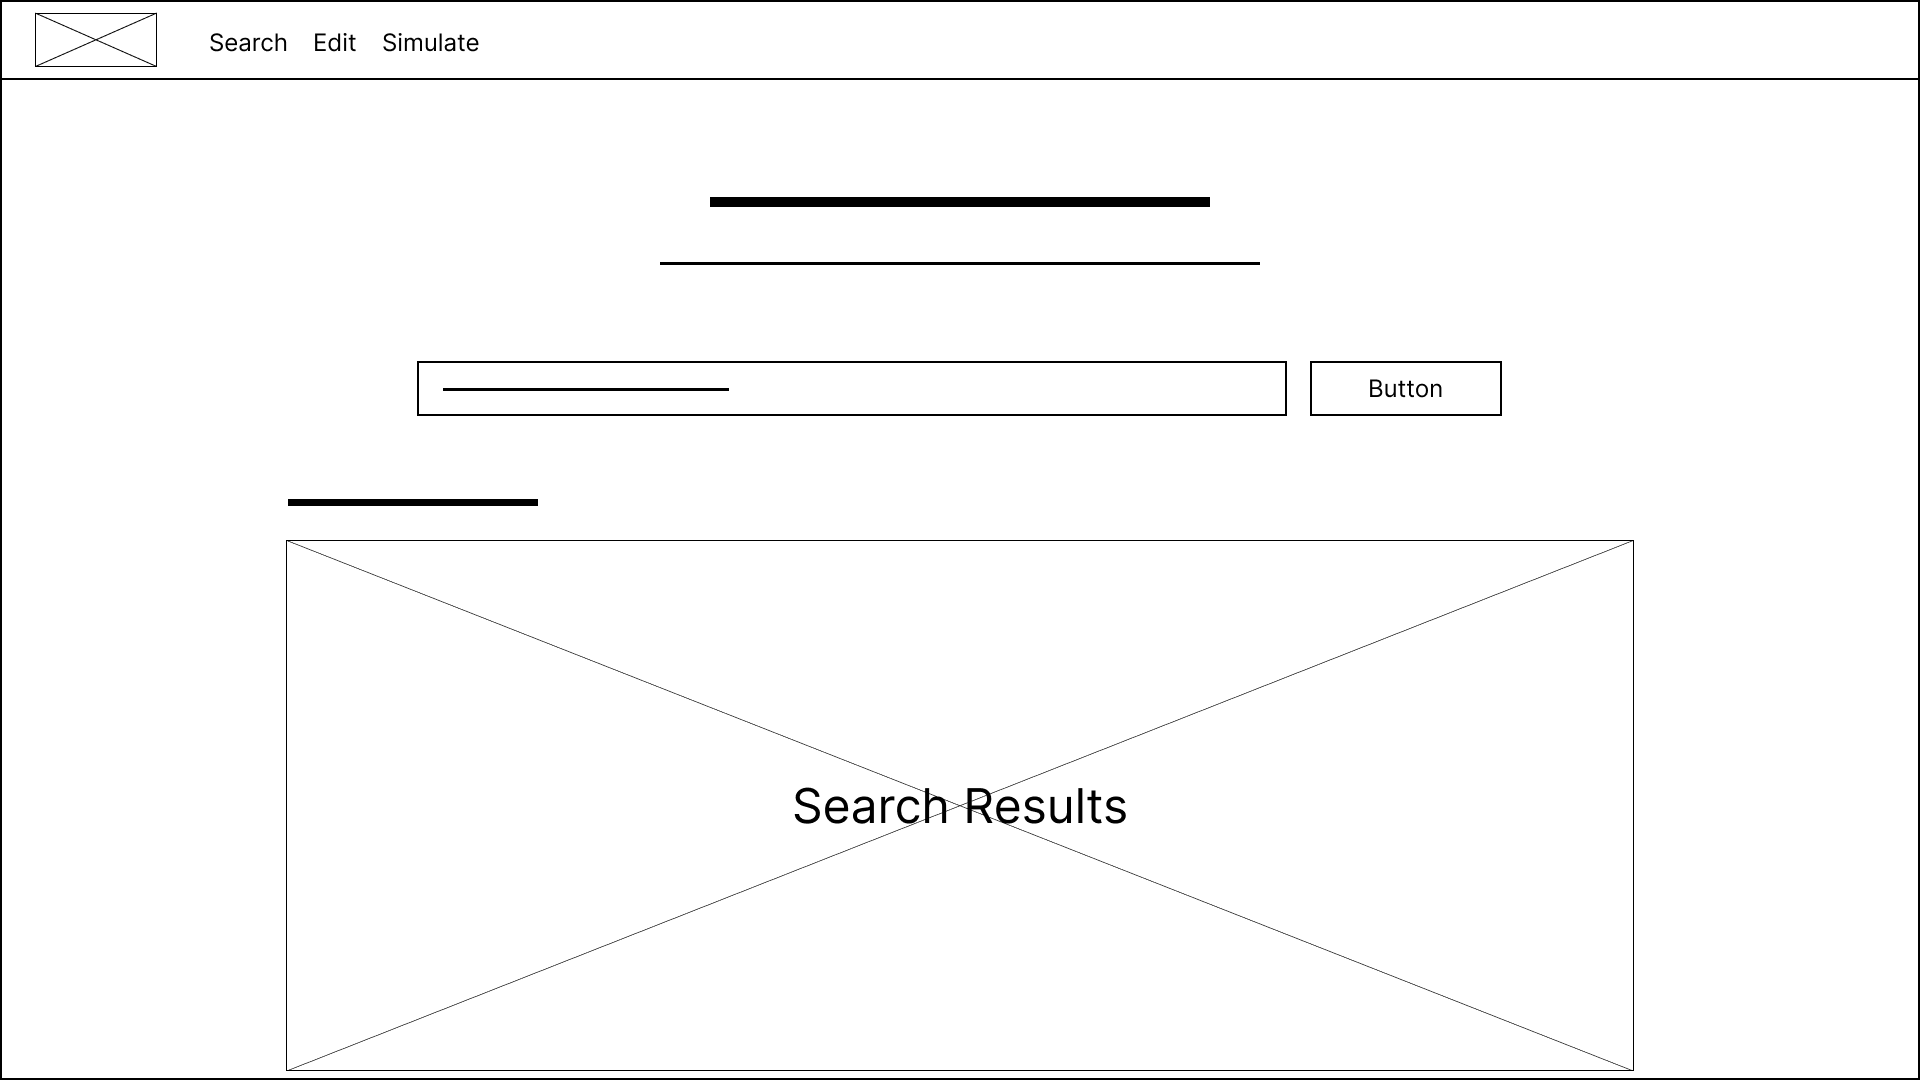
\includegraphics[width=\columnwidth]{media/lofi-search-tab.png}
    \caption{{Low-fidelity wireframe of the search interface.}}
    \label{fig:design:lofi_search}
\end{figure}

The editor workspace shown in Figure~\ref{fig:design:lofi_edit} combines the elements required for program comprehension and modification within a single interface. The workspace consists of a main program view for the structured program representation, a structural navigation view for exploring program elements at a higher level of abstraction and helping the user build a mental model of the program, and an assistant panel for contextual explanation and support. Integrating these capabilities within the same workspace is a deliberate design decision intended to reduce fragmentation between program inspection, navigation, and assistant interaction during iterative development tasks.

\begin{figure}[H]
    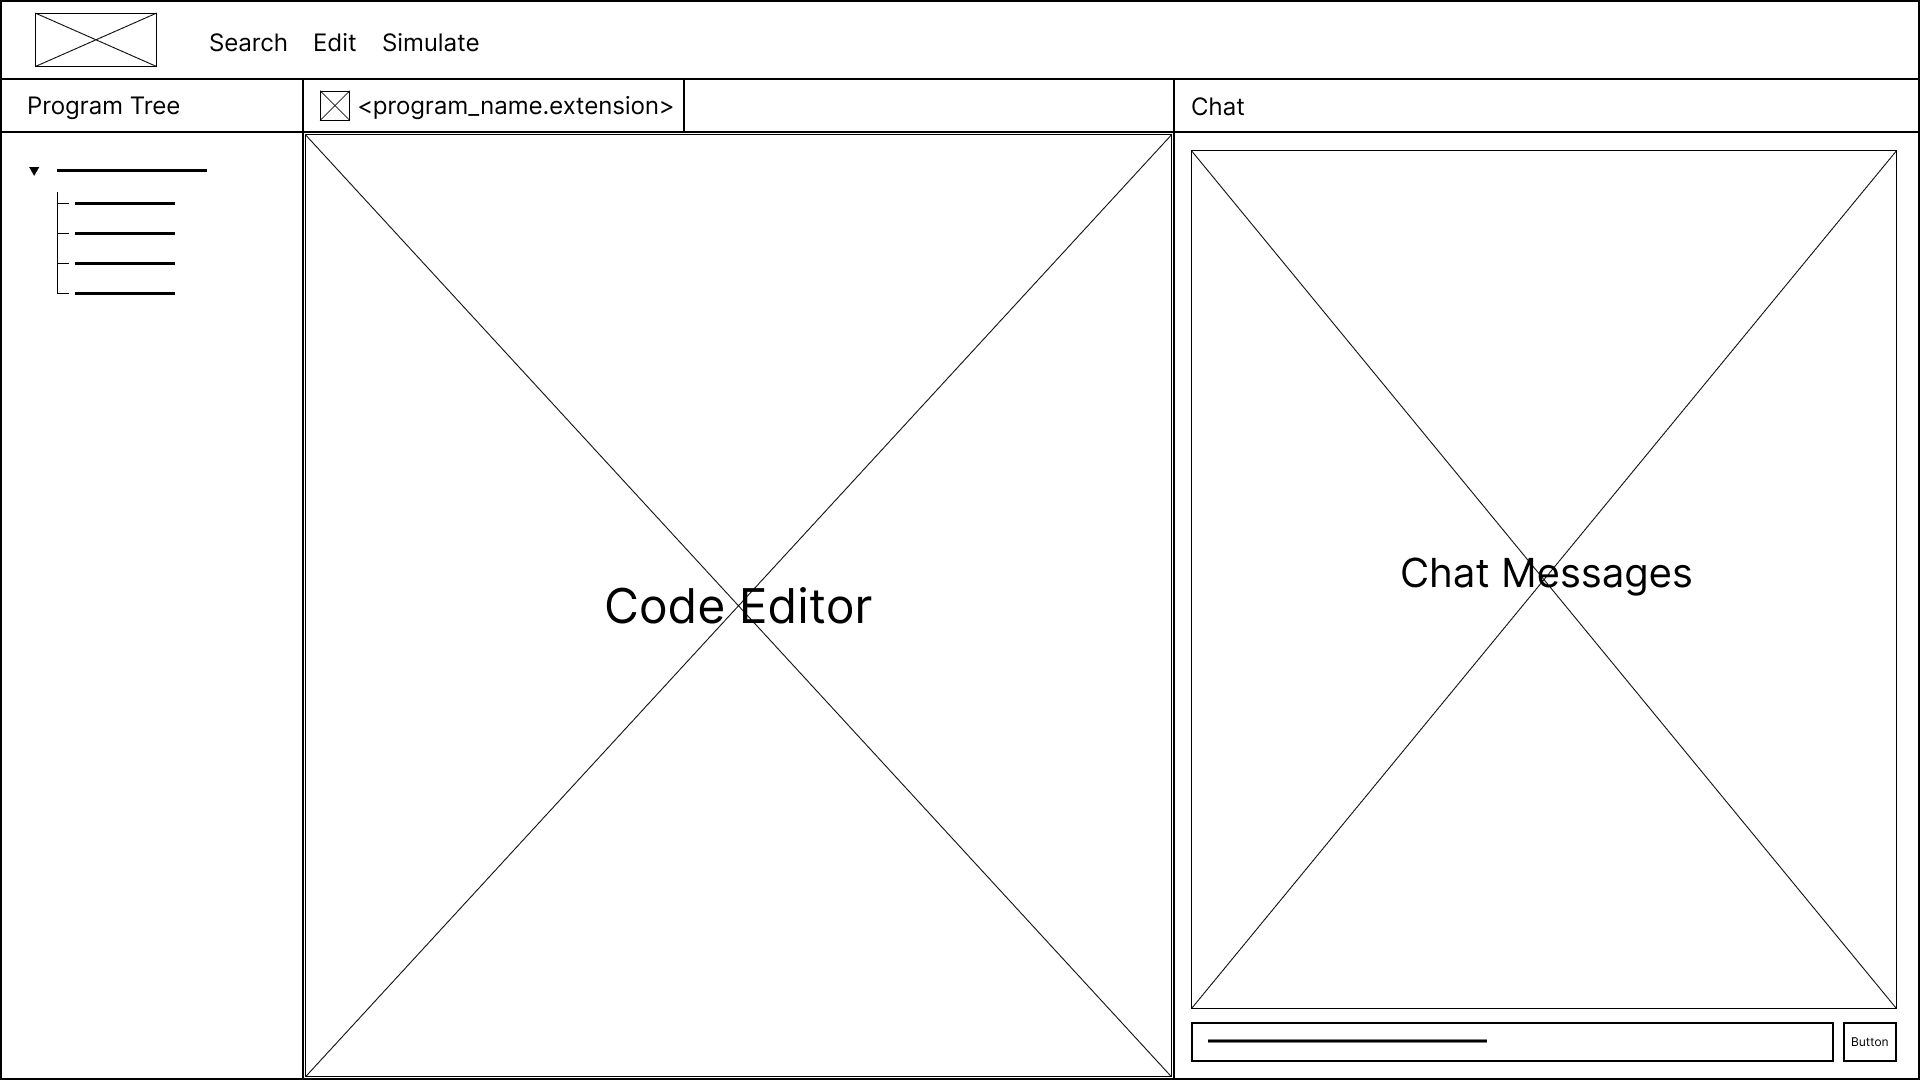
\includegraphics[width=\columnwidth]{media/lofi-edit-tab.png}
    \caption{{Low-fidelity wireframe of the edit interface.}}
    \label{fig:design:lofi_edit}
\end{figure}

The frontend should also preserve interaction state across workspaces. When a user transitions from the search workspace to the editor workspace, the selected program, search context, and assistant context should remain available. The client application should therefore maintain shared application state for the active program, program modifications, and conversational context throughout the interaction workflow.


\section{Client-Server Interaction}
The frontend should communicate with the backend through a REST-based API. A REST architecture provides a clear separation between user-interface concerns and backend functionality such as retrieval, artifact management, and language-model orchestration. This separation improves modularity and allows frontend and backend components to evolve independently through well-defined interfaces.

A REST-based design is also well suited to the interaction patterns of the system. Operations such as searching for robotic programs, retrieving artifacts, and submitting assistant requests naturally follow a request-response structure, making REST an appropriate and lightweight integration approach.

Using standard HTTP-based communication additionally simplifies interoperability with external systems and future extensions of the platform. It also allows the frontend to remain independent of backend implementation details, which supports maintainability and flexibility as the assistant architecture evolves.

Figure \ref{fig:design:search_sequence} shows the communication pattern for program discovery using semantic search. The client should submit a natural-language query through \texttt{POST /api/search}, after which the REST API should obtain a query embedding and use it to search the \texttt{program\_metadata} collection in the vector database. This is an important design distinction: the search interaction should operate over metadata-oriented vector representations, not over the full program code. The response should therefore contain ranked, discovery-oriented results together with the associated \texttt{program\_id}, rather than complete program artifacts. A design in which the full program is attached as metadata for each embedding was considered, but rejected because it would increase payload size, reduce responsiveness during result exploration, and weaken the separation between semantic retrieval and artifact access. Search failure should likewise remain explicit at the API boundary, so the client can present a clear error state to the user.

\begin{figure}[H]
    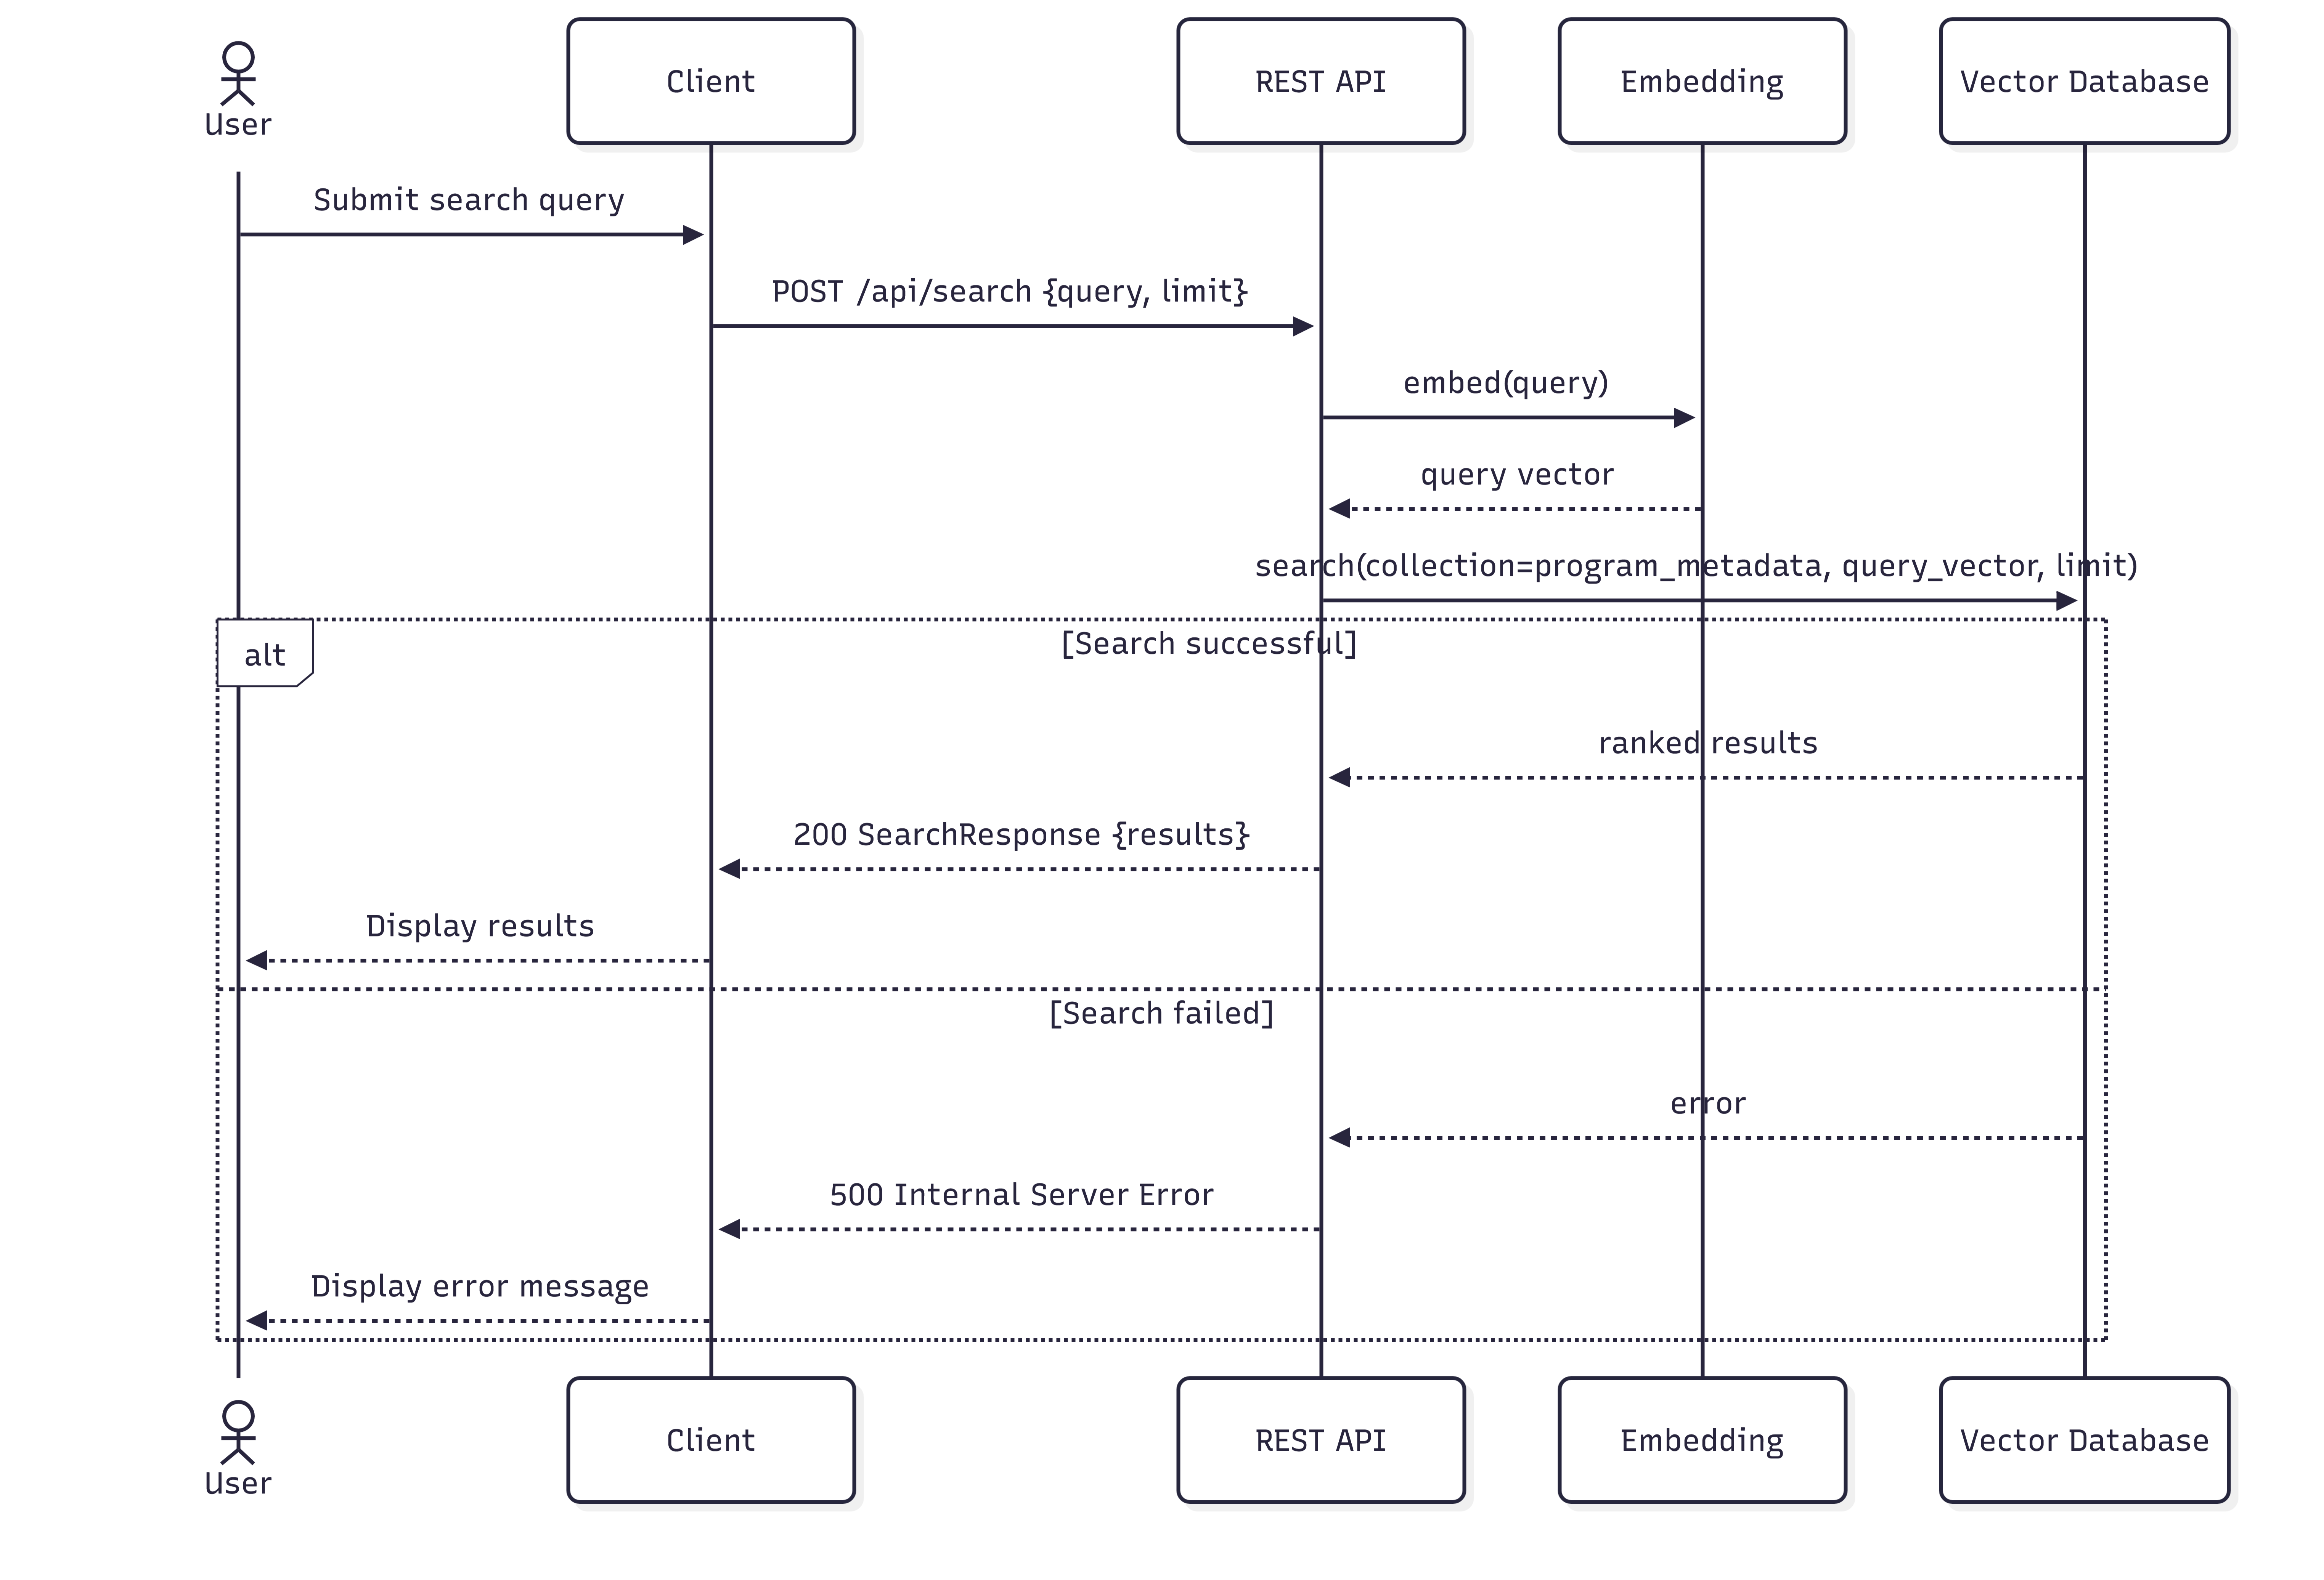
\includegraphics[width=\columnwidth]{media/search-sequence-diagram.png}
    \caption{{Sequence diagram illustrating the communication flow for the search functionality in the robot program editor.}}
    \label{fig:design:search_sequence}
\end{figure}

Once the user selects a program, the frontend should transition to the editor workspace and request the complete artifact through \verb|GET /api/programs/{program_id}/json|, as illustrated in Figure \ref{fig:design:loadProgram_sequence}. The API should resolve this request by calling \texttt{get\_program(program\_id)} on the ProgramStore and returning the corresponding \texttt{program\_json} when the program is found, or a not-found response otherwise. This two-stage interaction reflects a deliberate architectural separation between retrieval and artifact access. The ProgramStore should be a minimal artifact store keyed by \texttt{program\_id}, with the full program representation \texttt{program\_json} held separately from the vector collection. The same \texttt{program\_id} should therefore also be preserved as linking metadata in the search results, allowing a program discovered through semantic search over metadata to be resolved to the stored program artifact used by the editor.

\begin{figure}[H]
    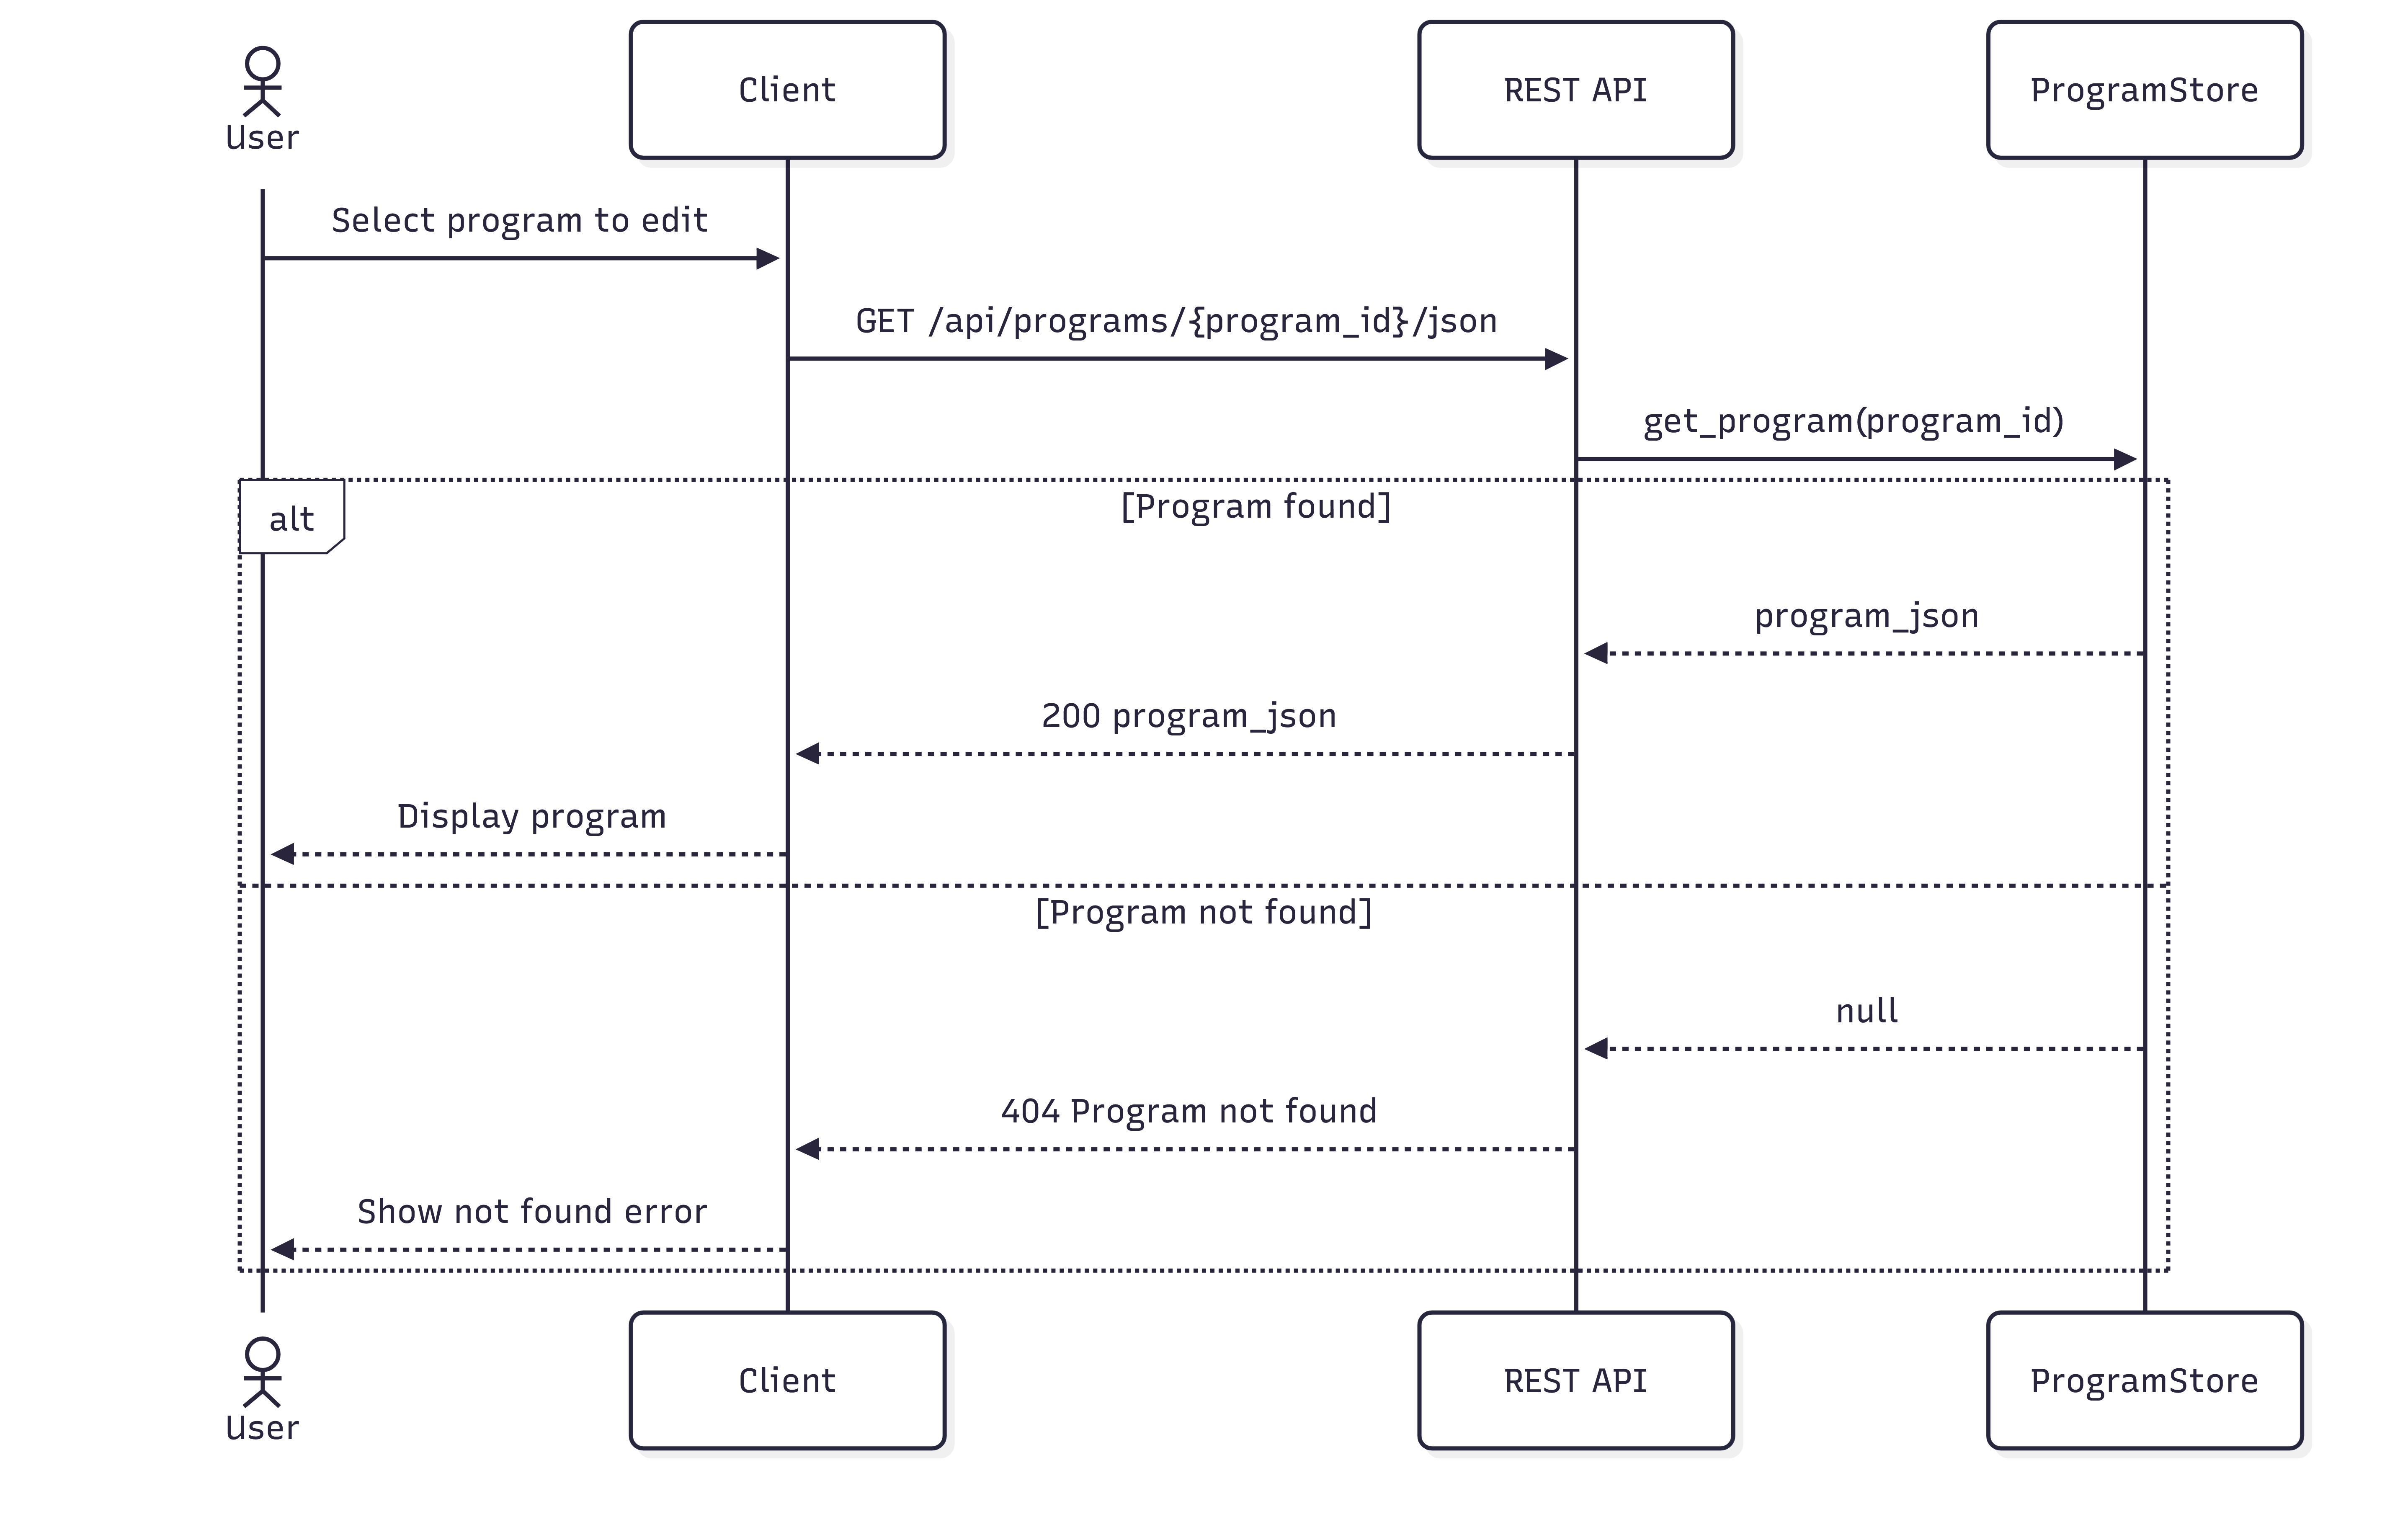
\includegraphics[width=\columnwidth]{media/loadProgram-sequence-diagram.png}
    \caption{{Sequence diagram illustrating the communication flow for the load program functionality in the robot program editor.}}
    \label{fig:design:loadProgram_sequence}
\end{figure}

% \begin{figure}[H]
%     \centering
%     \includegraphics[width=0.3\columnwidth]{media/programStore-table.png}
%     \caption{{ProgramStore schema.}}
%     \label{fig:design:programStore_table}
% \end{figure}

Figure \ref{fig:design:chat_sequence} illustrates the assistant interaction within the editor workspace. The client should submit chat requests through \texttt{POST /api/chat} together with the user message and optional program context derived from the currently loaded artifact. The orchestrator is responsible for agentic assistant functionality, including the loop of up to \texttt{max\_steps}. In each step, the tool-enabled agent should use the language model to decide whether retrieval is needed, use the embedding component and vector database when relevant tool calls are required, and then generate a final response from the gathered context.

\begin{figure}[H]
    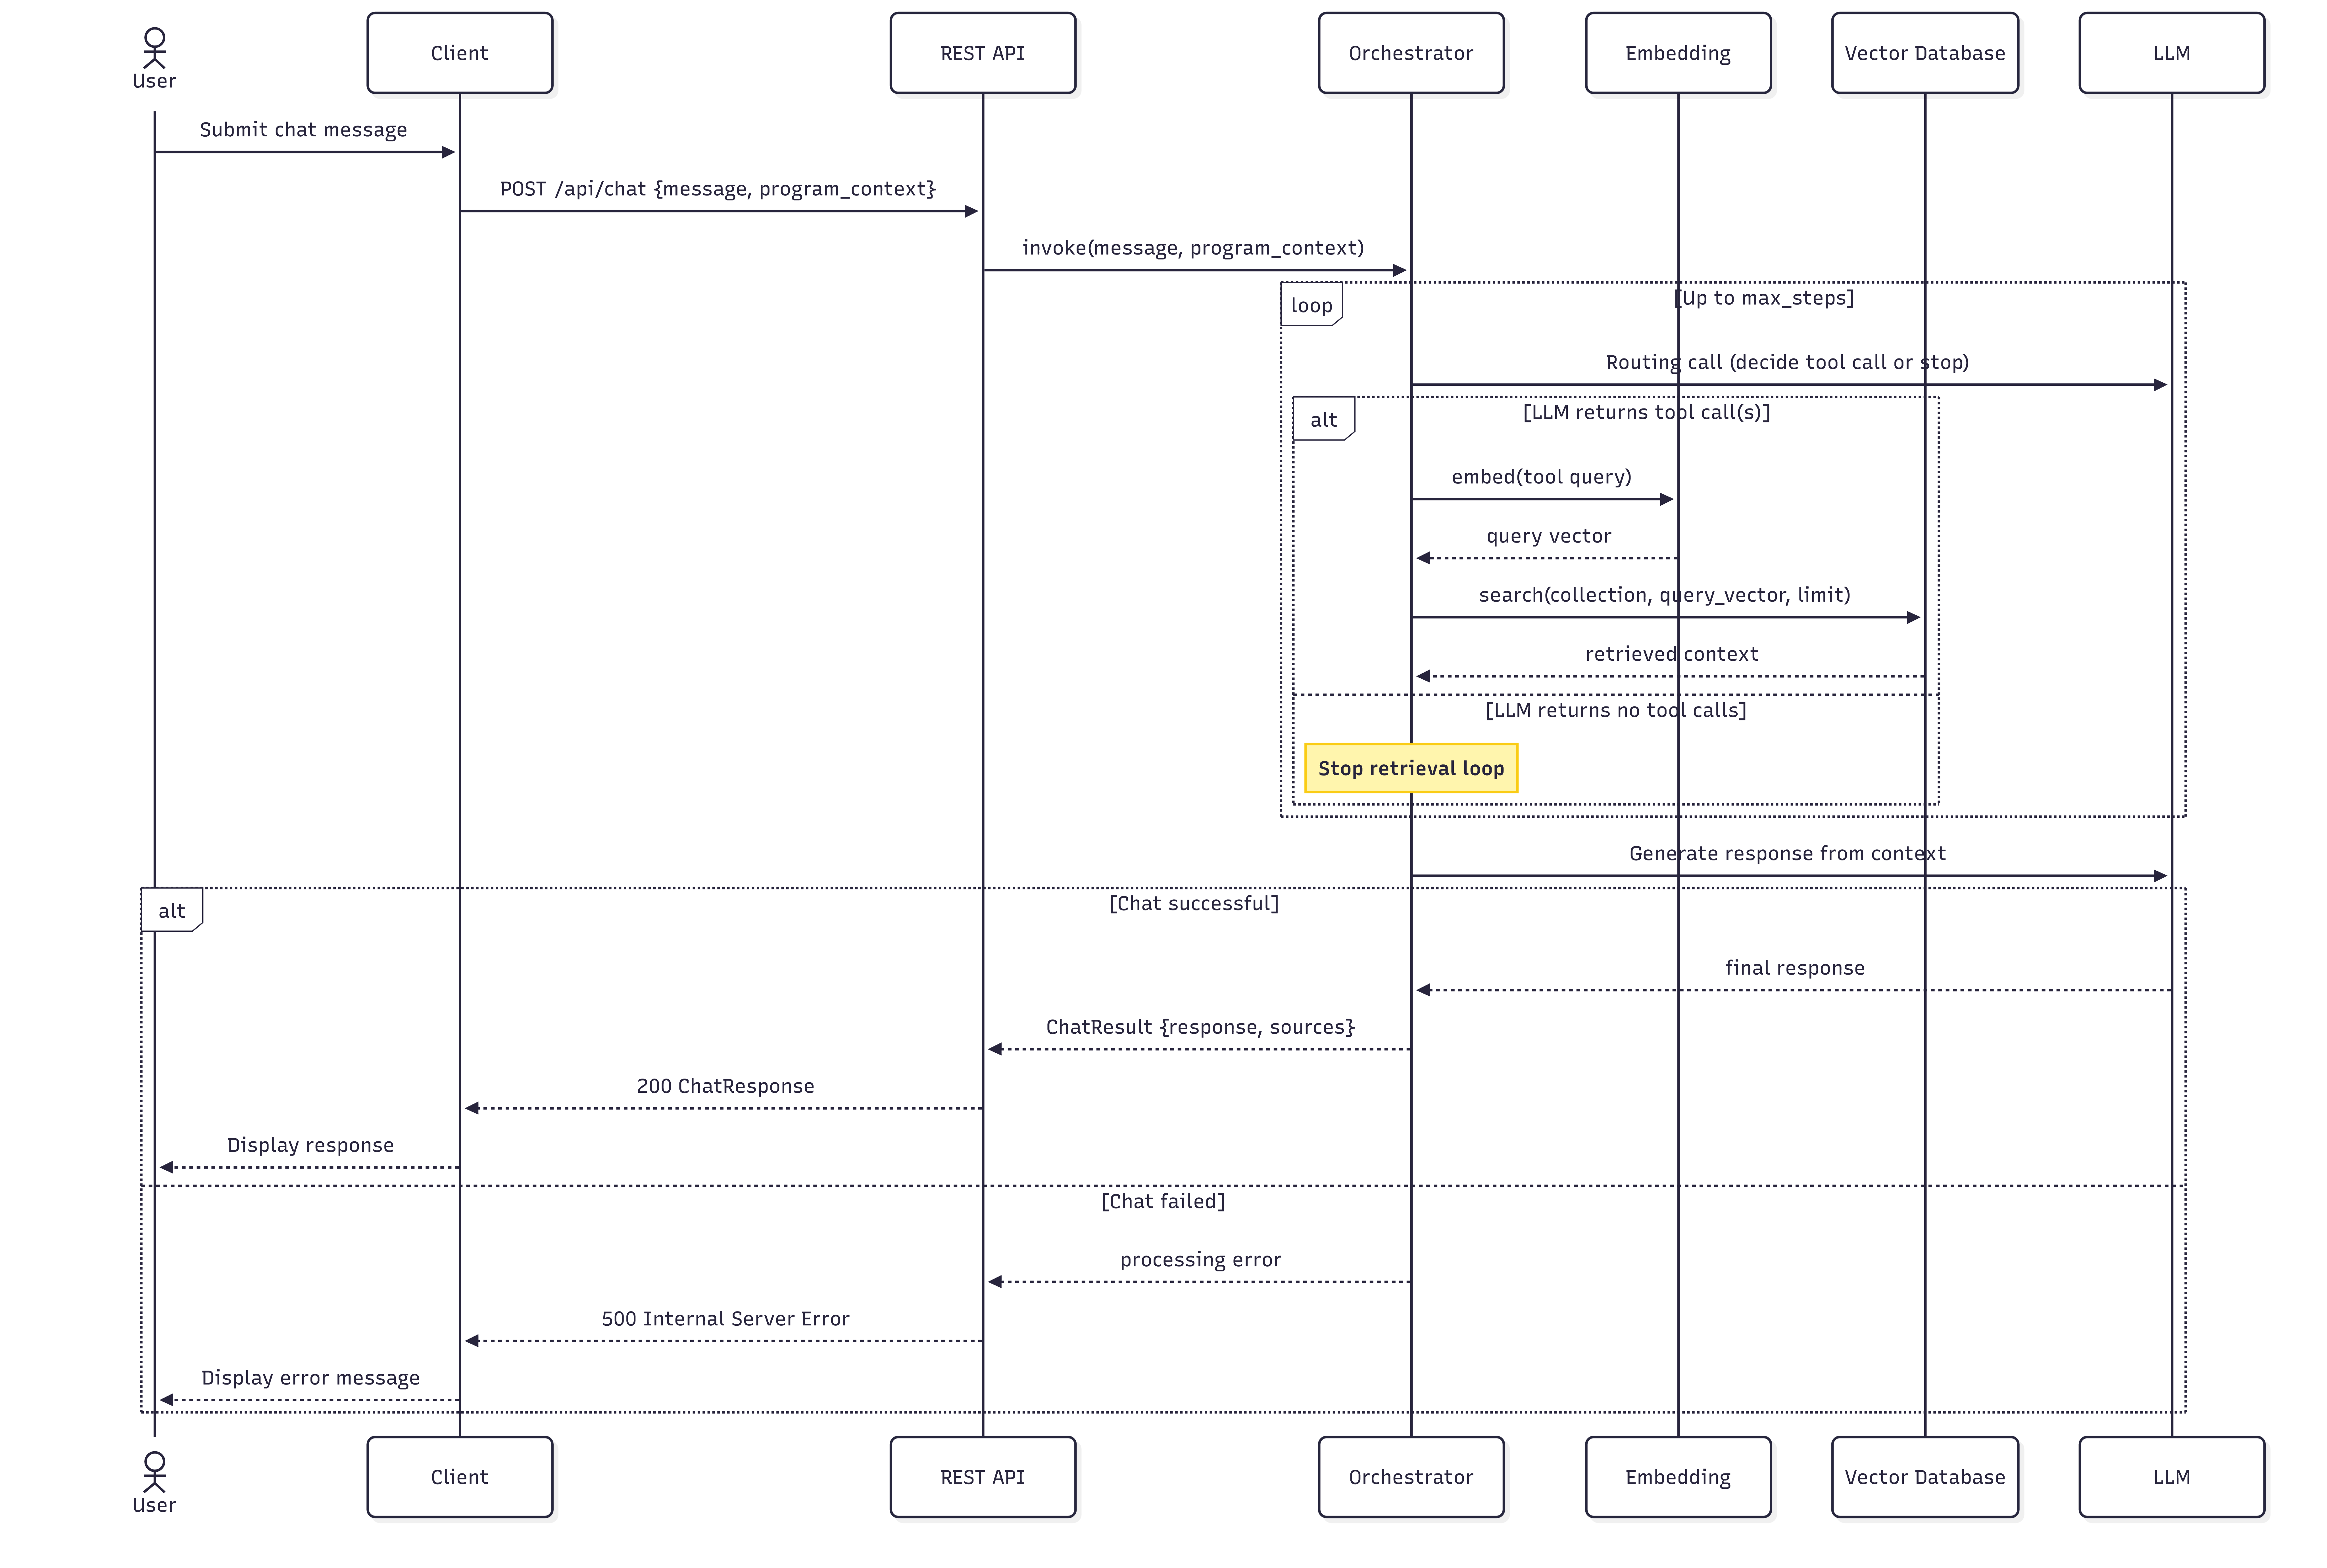
\includegraphics[width=\columnwidth]{media/chat-sequence-diagram.png}
    \caption{{Sequence diagram illustrating the communication flow for the chat functionality in the robot program editor.}}
    \label{fig:design:chat_sequence}
\end{figure}


\section{Technologies}
This section discusses the primary technology choices made for the system implementation and the considerations that motivated these selections.

\subsection{Backend}
The backend is responsible for retrieval orchestration, language-model interaction, data management, and communication with the frontend. The implementation should support rapid development, strong ecosystem support for AI tooling, and integration with modern machine-learning infrastructure.

Python was selected as the backend programming language. Python is widely adopted within the AI and machine-learning community and provides mature libraries and frameworks for AI development. This significantly reduces implementation complexity and improves compatibility with emerging AI infrastructure. While languages such as Java, C++, or Go may provide stronger performance characteristics, Python offers a more suitable balance between development efficiency, ecosystem maturity, and rapid research-oriented experimentation for the scope of this project.

\subsubsection{AI Infrastructure and Orchestration}
The assistant orchestration layer should support tool invocation, retrieval workflows, prompt management, and integration with language models. Several orchestration frameworks exist for LLM-based systems, including LangChain, LlamaIndex, and custom orchestration pipelines.

The project adopts LangChain, as the orchestration framework. LangChain provides abstractions for tool-based reasoning, retrieval workflows, prompt composition, and conversational interaction, which align well with the ReAct-inspired assistant architecture adopted in the project. LangChain simplifies integration between language models, retrieval pipelines, and external tools while remaining sufficiently flexible for experimentation with orchestration logic.

Alternative approaches based on fully custom orchestration pipelines would provide greater architectural control and potentially lower abstraction overhead. However, they would also require substantially more implementation effort for functionality already provided by existing frameworks.

For language-model serving, the system adopts Ollama. Ollama provides a lightweight local inference environment for running language models through a standardized interface. This simplifies experimentation with different models. Running models locally reduces dependence on external cloud services and avoids expensive API usage. Cloud-hosted APIs remain a relevant alternative, particularly for accessing larger models, but local model hosting is sufficient for development and experimentation.

\subsubsection{Storage}
The system requires storage for both semantic retrieval and structured artifact management. These requirements are handled through separate storage technologies optimized for their respective workloads.

For semantic retrieval, the project adopts Qdrant as the vector database. Vector databases are specifically designed for efficient similarity search in high-dimensional embedding spaces and therefore align naturally with the retrieval requirements of retrieval-augmented generation systems. Qdrant provides efficient vector indexing, metadata filtering, and good integration with Python-based AI tooling. Alternative vector databases such as ChromaDB, Pinecone, or Weaviate were also relevant options. However, Qdrant offers a lightweight self-hosted deployment model together with strong retrieval performance and mature ecosystem support.

Structured program artifacts and metadata should be stored separately from vector embeddings. For this purpose, the project adopts SQLite as the primary artifact store. SQLite provides a lightweight relational database with minimal deployment complexity while still supporting structured queries, indexing, and transactional consistency. For the scale and scope of this project, SQLite provides sufficient performance without introducing the operational overhead associated with larger database systems such as PostgreSQL or MySQL.

\subsubsection{Communication}
Communication between frontend and backend components should be exposed through a REST-based API. The backend API framework should therefore support asynchronous request handling, structured data validation, and integration with the Python-based backend infrastructure.

The project adopts FastAPI as the backend API framework. FastAPI provides a lightweight and modern framework for building REST APIs in Python with support for asynchronous operations and automatic request validation. These features simplify implementation of conversational AI endpoints and retrieval-oriented APIs while integrating naturally with the existing backend.

Alternative frameworks such as Flask or Django were also considered. Flask provides a simpler and highly flexible framework, while Django offers a more comprehensive full-stack architecture. However, FastAPI provides a good balance between lightweight design and modern API-oriented development for the needs of this project.


\subsection{Frontend}
The frontend should support interactive assistant workflows, program inspection, and workspace navigation while remaining responsive and extensible. The implementation therefore benefits from technologies that support component-based user interfaces and dynamic client-side interaction.

The project adopts React as the frontend framework. React provides a component-based architecture that aligns well with the modular structure of the interface, including separate search, editor, and assistant views. Its reactive rendering model is also well suited for AI-assisted interaction such as conversational interfaces.

Alternative frontend frameworks such as Angular or Vue were also relevant options. Angular provides a more opinionated full-framework architecture, while Vue offers a lightweight and approachable component model. However, React was selected due to its broad ecosystem support, flexibility, and widespread adoption within modern web application development.

The frontend additionally adopts React Router for client-side navigation between application workspaces. Since the interface separates search-oriented workflows from program comprehension and modification workflows, client-side routing provides a structured way to manage navigation and preserve interaction state across views without requiring full page reloads. This supports a smoother and more application-like user experience during iterative development tasks.

For program editing and inspection, the frontend adopts the Monaco Editor, which provides the editor infrastructure used in Visual Studio Code. Monaco offers features such as syntax highlighting, structured code editing, and extensibility for future language-support capabilities. This makes it well suited for robotic program inspection and modification tasks, where readability and structured interaction with program artifacts are important.
